\documentclass[a4paper,12pt]{article}
\usepackage{../packages/coursCollege}
\newcommand{\Chapitre}{Dérivation}
\renewcommand{\path}{../../}

\renewcommand{\cours}{3MA1~--~EG~--~ns~--~2025-2026}
\begin{document}

\section{Activités}
\begin{activite}
Introduction géométrique à la notion de limite	
	\tcblower

Vous disposez d’un stock de plaques rectangulaires au contour rigide, mesurant 1,2 mètres de large et 2 mètres de long. Pour votre prochain déménagement, vous désirez construire des cartons, ouverts vers le haut (en forme de parallélépipèdes rectangles) selon le procédé suivant : on découpe dans les quatre coins de la plaque le même carré, puis on plie les côtés et on les scotche pour former la boîte.

\hfill
\begin{minipage}[t]{0.4\textwidth}{
\vspace{0pt}
\begin{tikzpicture}[>=latex]
  % dimensions
  \def\W{4}   % correspond à 2 m
  \def\H{2.4} % correspond à 1,2 m
  \def\x{0.6} % côté du carré découpé

  % plaque avec coins découpés
  \draw (0,0) rectangle (\W,\H);
  \draw[dashed] (0,0) -- (\x,0) -- (\x,\x) -- (0,\x) -- cycle;
  \draw[dashed] (\W,0) -- (\W-\x,0) -- (\W-\x,\x) -- (\W,\x) -- cycle;
  \draw[dashed] (0,\H) -- (\x,\H) -- (\x,\H-\x) -- (0,\H-\x) -- cycle;
  \draw[dashed] (\W,\H) -- (\W-\x,\H) -- (\W-\x,\H-\x) -- (\W,\H-\x) -- cycle;

  % cotes
  \draw[<->] (0,-0.5) -- (\W,-0.5) node[midway,below]{$2\mathrm{\,m}$};
  \draw[<->] (\W+0.5,0) -- (\W+0.5,\H) node[midway,right]{$1{,}2\mathrm{\,m}$};
\end{tikzpicture}

}
\end{minipage}
\begin{minipage}[t]{0.4\textwidth}{
\vspace{0pt}
\begin{tikzpicture}[>=latex]
  % plan du carton (réseau)
  \def\W{3.4}
  \def\H{1.8}
  \def\x{0.6}

  % face centrale
  \draw (0,0) rectangle (\W,\H);
  % rabats
  \draw (0,\H) rectangle (\W,\H+\x);      % dessus
  \draw (0,-\x) rectangle (\W,0);         % dessous
  \draw (-\x,0) rectangle (0,\H);         % gauche
  \draw (\W,0) rectangle (\W+\x,\H);      % droite

  % lignes de pliage
  \draw[dashed] (0,0) -- (\W,0);
  \draw[dashed] (0,\H) -- (\W,\H);
  \draw[dashed] (0,0) -- (0,\H);
  \draw[dashed] (\W,0) -- (\W,\H);
\end{tikzpicture}
}
\end{minipage}
\hfill

Comment obtenir des cartons de volume maximal ?
\end{activite}
\begin{activite}
	\tcblower

Une population de 25\,000 individus (au temps $t=0$) croît selon la formule
\[
  N(t)
  = 25000 + 45\,t^2,
\]
où $t$ est mesuré en jours.

\begin{tasks}
  \task Calculer la vitesse moyenne à laquelle croît la population entre les instants donnés :
  \begin{multicols}{3}	
    \begin{enumerate}
      \item $t_1 = 0$ et $t_2 = 2$
      \item $t_1 = 2$ et $t_2 = 3$
      \item $t_1 = 1$ et $t_2 = 4$
      \item $t_1 = 2$ et $t_2 = 5$
    \end{enumerate}
\end{multicols}
  \task Calculer la vitesse instantanée de la croissance à l’instant $\displaystyle t = 2$.
\end{tasks}
\end{activite}

\begin{activite}
\tcblower
On considère la fonction $f$ définie par
\[
  f(x) = 2x^2 - 1.
\]

\begin{tasks}(1)
  \task Quel est le taux (moyen) de variation entre :
  \begin{multicols}{2}	
    \begin{enumerate}
      \item $(0; f(0))$ et $(2; f(2))$ ?
      \item $(0; f(0))$ et $(1; f(1))$ ?
    \end{enumerate}
  \end{multicols}
  \task Quel est le taux instantané de variation en :
  \begin{multicols}{3}	
    \begin{enumerate}
      \item $(0; f(0))$ ?
      \item $(1; f(1))$ ?
      \item $(2; f(2))$ ?
    \end{enumerate}
  \end{multicols}
  \task Que peut-on dire de la pente de la droite tangente à la courbe représentative de $f$ en :
  \begin{multicols}{3}	
    \begin{enumerate}
      \item $(0; f(0))$ ?
      \item $(1; f(1))$ ?
      \item $(2; f(2))$ ?
    \end{enumerate}
\end{multicols}
\end{tasks}

Interpréter graphiquement l’exercice.
\end{activite}

\begin{activite}{Nombre dérivé}
\tcblower
On considère la fonction \(f\) définie par
\[
  f(x)=\dfrac{1}{2x}.
\]
\begin{tasks}(1)
  \task Calculer le taux de variation de la fonction \(f\) entre deux points d’abscisses 1 et \(x\).
  \task Calculer le nombre dérivé de la fonction \(f\) en 1 et interpréter graphiquement.
\end{tasks}
\end{activite}

\begin{activite}{Toujours possible ?}
\tcblower
On considère la fonction \(f\) définie par
\[
  f(x)=\lvert x-1\rvert.
\]
\begin{tasks}(1)
  \task Représenter graphiquement cette fonction.
  \task Estimer graphiquement \(f'(2)\) et \(f'(0)\).
  \task Calculer \(f'(2)\) et \(f'(0)\).
  \task Estimer graphiquement \(f'(1)\).
  \task Calculer \(f'(1)\).
  \task Comment s’exprime graphiquement une situation de non dérivabilité ?
\end{tasks}
\end{activite}

\begin{activite}{Fonction dérivée}
\tcblower
On considère la fonction \(f\) définie par
\[
  f(x)=\dfrac{1}{2x}.
\]
\begin{tasks}(1)
  \task Calculer le taux de variation de la fonction \(f\) entre deux points d’abscisses \(a\) et \(x\).
  \task Calculer le nombre dérivé de la fonction \(f\) entre deux points d’abscisses \(a\) et \(x\). On obtient une nouvelle fonction : la dérivée de \(f\).
  \task Existe-t-il un point du graphe de \(f\) en lequel la tangente à la courbe représentative de \(f\) (ou par raccourci « à \(f\) ») soit horizontale ? Justifier et interpréter graphiquement.
  \task En quel(s) point(s) du graphe de \(f\) la pente de la tangente à \(f\) est-elle égale à \(-\dfrac{1}{12}\) ?
\end{tasks}
\end{activite}

\begin{activite}{Notations}
\tcblower
On considère la fonction \(f\) définie par
\[
  f(x)=x^2-1.
\]
\begin{tasks}(1)
  \task Déterminer la dérivée de \(f\) en \(a\).
  \task Interpréter graphiquement.
  \task Considérer \(x\) et \(x+h\) au lieu de \(a\) et \(x\) et déterminer la dérivée de \(f\) en \(x\).
\end{tasks}
\end{activite}

\begin{activite}{Équation de la tangente}
\tcblower
On considère une fonction dérivable en \((a;f(a))\) et on s’intéresse à la tangente à (la courbe représentative de) \(f\) en \((a;f(a))\). Écrire une conjecture quant à son équation, l’illustrer et la démontrer.
\end{activite}

\begin{activite}{Tangentes extérieures}
\tcblower
On considère la fonction \(f\) définie par
\[
  f(x)=\dfrac{x^4}{x+5}.
\]
\begin{tasks}(1)
  \task Déterminer les coordonnées d’un point \(P\) tel que la tangente à la courbe représentative de \(f\) au point \(P\) passe par l’origine \((0;0)\) du repère (s’il y a plusieurs solutions, les trouver toutes).
  \task Vérifier graphiquement en représentant la courbe et les tangentes trouvées.
\end{tasks}
\end{activite}


\begin{activite}{Graphiquement}
\tcblower
\begin{tasks}(1)
  \task Parmi les fonctions représentées ci-dessous, certaines sont dérivées d’une autre. Il s’agit de les retrouver :
\end{tasks}
\begin{center}
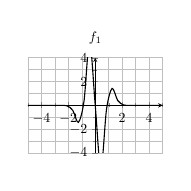
\begin{tikzpicture}[scale=0.5]
  \begin{axis}[
    title={$f_1$},
    xmin=-5, xmax=5, ymin=-4, ymax=4,
    axis lines=middle, grid=both, minor tick num=1,
    width=5cm, height=4cm
  ]
    \addplot[smooth,thick] {(32*x^3 - 24*x)*exp(-2*x^2)};
  \end{axis}
\end{tikzpicture}\quad
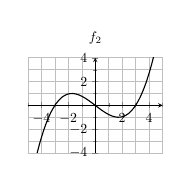
\begin{tikzpicture}[scale=0.5]
  \begin{axis}[
    title={$f_2$},
    xmin=-5, xmax=5, ymin=-4, ymax=4,
    axis lines=middle, grid=both, minor tick num=1,
    width=5cm, height=4cm
  ]
    \addplot[smooth,thick] {(x^3 - 9*x)/(6*sqrt(3))};
  \end{axis}
\end{tikzpicture}\quad
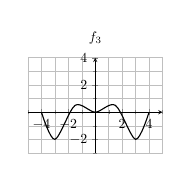
\begin{tikzpicture}[scale=0.5]
  \begin{axis}[
    title={$f_3$},
    xmin=-5, xmax=5, ymin=-3, ymax=4,
    axis lines=middle, grid=both, minor tick num=1,
    width=5cm, height=4cm
  ]
    \addplot[smooth,thick] coordinates {
      (-4,0) (-3,-2) (-1.5,0.5) (0,0) (1.5,0.5) (3,-2) (4,0)
    };
  \end{axis}
\end{tikzpicture}

\vspace{1em}

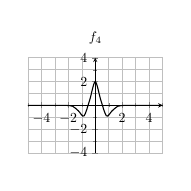
\begin{tikzpicture}[scale=0.5]
  \begin{axis}[
    title={$f_4$},
    xmin=-5, xmax=5, ymin=-4, ymax=4,
    axis lines=middle, grid=both, minor tick num=1,
    width=5cm, height=4cm
  ]
    \addplot[smooth,thick] {4*(0.5 - 2*x^2)*exp(-2*x^2)};
  \end{axis}
\end{tikzpicture}\quad
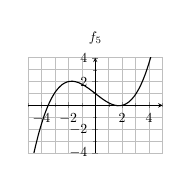
\begin{tikzpicture}[scale=0.5]
  \begin{axis}[
    title={$f_5$},
    xmin=-5, xmax=5, ymin=-4, ymax=4,
    axis lines=middle, grid=both, minor tick num=1,
    width=5cm, height=4cm
  ]
    \addplot[smooth,thick] {((x+3.5)*(x-1.5)*(x-2))/10.5};
  \end{axis}
\end{tikzpicture}\quad
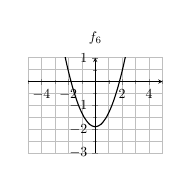
\begin{tikzpicture}[scale=0.5]
  \begin{axis}[
    title={$f_6$},
    xmin=-5, xmax=5, ymin=-3, ymax=1,
    axis lines=middle, grid=both, minor tick num=1,
    width=5cm, height=4cm
  ]
    \addplot[smooth,thick] {0.58642*(x^2 - 3.24)};
  \end{axis}
\end{tikzpicture}
\end{center}
\end{activite}


\begin{activite}{Vrai ou faux ?}
\tcblower
Vrai ou faux ? Justifier.
\begin{tasks}(1)
  \task Si \(f\) est une fonction définie sur un intervalle ouvert \(I\) et si \(a\in I\), alors \(f\) est dérivable en \(a\).
  \task Soit \(f\) la fonction définie par \(f(x)=x^2\). Si \(a\) et \(b\) sont deux nombres réels quelconques, alors le taux de variation moyen de \(f\) entre \(a\) et \(b\) est égal à \(f'\left(\dfrac{a+b}{2}\right)\).
\end{tasks}
\end{activite}

\begin{activite}{Formules de dérivation}
\tcblower
\begin{enumerate}
  \item Rappels de fonctions élémentaires dont on a calculé la dérivée à l’aide de la définition :
	  \begin{multicols}{3}	  	
    \begin{itemize}
      \item [D1] \(\mathrm{cte}'=0\)
      \item [D2] \((x)'=1\)
      \item [D3] \((ax+b)'=a\)
      \item [D4] \((x^2)'=2x\)
      \item [D5] \((ax^2+bx+c)'=2a\,x+b\)
      \item [D6] \((x^3)'=3x^2\)
      \item [D7] \(\left(\sqrt{x}\right)'=\dfrac{1}{2\sqrt{x}}\)
      \item [D8] \(\left(\tfrac{1}{x}\right)'=-\dfrac{1}{x^2}\)
    \end{itemize}
\end{multicols}
  \item Il est possible d’accélérer le calcul de \(f'(x)\), sans avoir besoin de passer par de fastidieux calculs de limites… Dans la table numérique, on trouve un formulaire de ce genre :
	  \begin{multicols}{2}	  	
    \begin{itemize}
      \item [PrD1] \([\mathrm{cte}\cdot f]'=\mathrm{cte}\cdot f'\)
      \item [PrD2] \([f+g]'=f'+g'\)
      \item [PrD3] \([f-g]'=f'-g'\)
      \item [PrD4] \([f\cdot g]'=f'\cdot g+f\cdot g'\)
      \item [PrD5] \(\left[\dfrac{1}{f}\right]'=-\dfrac{f'}{f^2}\)
      \item [PrD6] \(\left[\dfrac{f}{g}\right]'=\dfrac{f'\,g - f\,g'}{g^2}\)
      \item [PrD7] \(\left[\dfrac{\mathrm{cte}}{f}\right]'=-\mathrm{cte}\,\dfrac{f'}{f^2}\)
      \item [PrD8] \(\left[(f(x))^n\right]'=n\,[f(x)]^{n-1}\,f'(x),\;\forall n\in\mathbb{R}\)
      \item [PrD9] \(\left[g(f(x))\right]'=g'(f(x))\cdot f'(x)\)
    \end{itemize}
	  \end{multicols}
  Les utiliser pour calculer les dérivées des fonctions suivantes, en donnant les réponses sans racine au dénominateur et sans exposant numérique négatif ou fractionnaire :
    \begin{tasks}(2)
      \task \(f(x)=3x\)
      \task \(f(x)=ax+b\), avec \(a\in\mathbb{R}^*\) et \(b\in\mathbb{R}\)
      \task \(f(x)=ax^2+bx+c\), avec \(a\in\mathbb{R}^*\) et \(b,c\in\mathbb{R}\)
      \task \(f(x)=\dfrac{1}{x}\)
      \task \(f(x)=\sqrt{x^2+1}\)
      \task \(f(x)=\dfrac{1}{x^2+1}\)
      \task \(f(x)=\dfrac{\sqrt{x}}{x}\)
      \task \(f(x)=-\dfrac{2}{x^3}\)
    \end{tasks}
  \item Reprendre l’activité 1 et la résoudre en utilisant les formules de dérivation.
  \item On considère la fonction $f$ définie par \(f(x)=\dfrac{x^3}{3}-2x^2+3x\)
\begin{tasks}(1)
  \task Calculer la dérivée de \(f\).
  \task Déterminer l’équation de la tangente au graphe de \(f\) au point \((0;0)\).
  \task Trouver un autre point du graphe de \(f\) en lequel la tangente est parallèle à la précédente.
  \task Déterminer les (deux !) coordonnées des points de la courbe représentative de \(f\) en lesquels la tangente est horizontale.
  \task Utiliser vos résultats pour tracer la courbe représentative de la fonction \(f\) et les tangentes trouvées aux questions b. et c.
\end{tasks}
\end{enumerate}
\end{activite}


\begin{activite}{Une dérivée importante}
\tcblower
On considère la fonction \(f\) définie par \(f(x)=x^n\), avec \(n\in\mathbb{R}\).
\begin{tasks}(1)
  \task Calculer \(f'(x)\) pour \(n=1\), \(n=2\), \(n=0\), \(n=0,5\).
  \task Énoncer une conjecture.
  \task* La démontrer dans les cas suivants :
  \begin{multicols}{2}
    \begin{enumerate}
      \item \(n\in\mathbb{N}^*\)
      \item \(n\in\mathbb{Z}_-\)
      \item \(n\) de la forme \(\dfrac{1}{m}\) avec \(m\in\mathbb{N}^*\)
      \item \(n\in\mathbb{Q}\)
    \end{enumerate}
  \end{multicols}
\end{tasks}
\end{activite}

\begin{activite}{Relation continuité-dérivabilité}
\tcblower
\begin{tasks}(1)
\task Explorer la relation entre continuité et dérivabilité en un point.
\task Énoncer un théorème puis le démontrer.
\task Que penser de la réciproque de ce théorème ?
\end{tasks}
\end{activite}
\begin{activite}{Démonstration des formules de dérivation}
\tcblower
\begin{tasks}(1)
\task Énoncer les formules de dérivation connues comme des théorèmes en identifiant clairement hypothèses et conclusions.
\task Démontrer les théorèmes pour $\alpha \cdot f$, $f + g$, $f \cdot g$, $\dfrac{1}{f}$.
\task Démontrer le théorème pour $\dfrac{f}{g}$.
\end{tasks}
\end{activite}
\begin{activite}
	Démonstration des formules de dérivation
	\tcblower
	Énoncer et démontrer la formule de dérivation de $x^n$ comme un théorème en identifiant clairement les hypothèses et conclusions.
\end{activite}

\begin{activite}{Dérivées trigonométriques}
\tcblower
\begin{tasks}(1)
\task Représenter graphiquement la fonction sin et sa dérivée sur un même repère.
\task Quelle conjecture quant à $[\sin(x)]'$ peut-on énoncer ?
\task Démontrer ce résultat.

Indication : utiliser la formule trigonométrique $\sin(a) - \sin(b) = 2\sin\left(\dfrac{a-b}{2}\right)\cos\left(\dfrac{a+b}{2}\right)$

\task Déterminer $[\cos(x)]'$ et $[\tan(x)]'$.
\end{tasks}
\end{activite}
\begin{activite}{Une nouvelle formule de dérivation}
\tcblower
\begin{tasks}(1)
\task Comment déterminer $[\sin(x^3)]'$ ? Quelle est l'opération considérée ici ?
\task Énoncer une nouvelle formule de dérivation.
\task Déterminer :
\begin{multicols}{2}
\begin{enumerate}
\item $[\sin(4x^4-2x)]'$
\item $[\sin^4(x)]'$
\item $[\cos^2(x)]'$
\item $[\tan^4(x^4-1)]'$
\item $[\sin^4(4x^4-2x)]'$
\item $[\sin(\sin(x))]'$
\end{enumerate}
\end{multicols}
\task Quelle relation y a-t-il entre cette nouvelle formule et $\|f(x)\|^n = n[f(x)]^{n-1} \cdot f'(x), \forall n \in \mathbb{R}$
\task Énoncer une formule pour déterminer $\sqrt{f(x)}$.
\end{tasks}
\end{activite}


\begin{activite}{Image d'un fermé}
\tcblower
On considère le théorème suivant : « Si $f: I \to \mathbb{R}$ est une fonction continue sur $[a,b]$, alors il existe $m$ et $M$ deux nombres réels tels que $f([a,b]) = [m;M]$ »

\begin{tasks}(1)
\task Faire un schéma pour interpréter graphiquement ce résultat.
\task Expliquer pourquoi on l'appelle le théorème « Image d'un fermé par une fonction continue ».
\task Illustrer (représentation graphique, qui sont $a$, $b$, $m$ et $M$ ?) ce théorème dans les cas suivants :
\begin{enumerate}
\item $f:[-1;1] \to \mathbb{R}$ déterminée par $f(x) = x^2$
\item $f:[1;100] \to \mathbb{R}$ déterminée par $f(x) = 2$
\item $f:[0;2] \to \mathbb{R}$ déterminée par $f(x) = x(x-2)^2$
\end{enumerate}
\task Que penser de la conjecture suivante : « Si $f: I \to \mathbb{R}$ est une fonction sur $[a,b]$, alors il existe $m$ et $M$ deux nombres réels tels que $f([a,b]) = [m;M]$ ». Qu'en déduire ?
\end{tasks}
\end{activite}
\begin{activite}{Théorème de Rolle}
\tcblower
On considère le théorème suivant : « Si $f: I \to \mathbb{R}$ est telle que $f$ est continue sur $[a,b]$, $f$ est dérivable sur $]a,b[$ et $f(a) = f(b)$, alors il existe au moins un nombre $c \in ]a,b[$ tel que $f'(c) = 0$ »

\begin{tasks}(1)
\task Faire un schéma pour interpréter graphiquement ce résultat.
\task Illustrer (représentation graphique, qui sont $a$, $b$ et $c$ ?) ce théorème dans les cas suivants :
\begin{enumerate}
\item $f:[-1;1] \to \mathbb{R}$ déterminée par $f(x) = x^2$
\item $f:[1;100] \to \mathbb{R}$ déterminée par $f(x) = 2$.
\item $f:[0;2] \to \mathbb{R}$ déterminée par $f(x) = x(x-2)^2$
\end{enumerate}
\task Discuter la pertinence des hypothèses.
\task * Pourquoi exige-t-on un intervalle ouvert pour la dérivabilité et un intervalle fermé pour la continuité ?
\task * Qui était Rolle ?
\task Démontrer le théorème de Rolle.
\end{tasks}
\end{activite}
\begin{activite}{Théorème des accroissements finis}
\tcblower
On considère le théorème suivant : « Si $f: I \to \mathbb{R}$ est telle que $f$ est continue sur $[a,b]$ et $f$ est dérivable sur $]a,b[$, alors il existe au moins un nombre $c \in ]a,b[$ tel que $f'(c) = \dfrac{f(b) - f(a)}{b - a}$ »

\begin{tasks}(1)
\task Faire un schéma pour interpréter graphiquement ce résultat.
\task Illustrer (représentation graphique, qui sont $a$, $b$ et $c$ ?) ce théorème dans les cas suivants :
\begin{enumerate}
\item $f:[-1;2] \to \mathbb{R}$ déterminée par $f(x) = x^2$
\item $f:[1;100] \to \mathbb{R}$ déterminée par $f(x) = 2$.
\item $f:[0;3] \to \mathbb{R}$ déterminée par $f(x) = x(x-2)^2$
\end{enumerate}
\task Discuter la pertinence des hypothèses.
\task Démontrer ce théorème.
\end{tasks}
\end{activite}
\begin{activite}{Application}
\tcblower
Trouver la ou les valeurs prévues par le théorème des AF pour la fonction $f$ définie par $f(x) = \sqrt{x}$ sur l'intervalle $[25;36]$.
\end{activite}
\begin{activite}{Corollaire du théorème des accroissements finis}
\tcblower
On considère le théorème suivant : « Soit $f$ définie sur un intervalle $I$. Alors on a :
\begin{itemize}
	\item si $f'(x) > 0, \forall x \in I$, alors $f$ est strictement croissante sur $I$
\item si $f'(x) < 0, \forall x \in I$, alors $f$ est strictement décroissante sur $I$
\item si $f'(x) = 0, \forall x \in I$, alors $f$ est constante sur $I$
\end{itemize}
\begin{tasks}(1)
\task Illustrer ce théorème.
\task À quoi est-il utile ?
\task Démontrer ce théorème.
\task Que penser de sa réciproque ?
\end{tasks}
\end{activite}


\begin{activite}{Extrema de \(f\) en \(a\) et dérivée \(f'(a)\)}
\tcblower
Nous avons vu que l’intention qui a justifié la construction de l’outil dérivée était la recherche d’extrema locaux d’une fonction donnée. Il s’agit maintenant d’aller au bout de cette démarche et d’expliciter le lien qui existe entre dérivée de \(f\) et extrema locaux de \(f'\).

\begin{tasks}(1)
  \task Donner une définition précise de la notion d’extremum global et local. Illustrer avec des exemples.
  \task Utiliser GeoGebra pour représenter des fonctions polynomiales et leur dérivée en explorant le lien supposé entre dérivée de \(f\) et extrema locaux de \(f'\).
  \task Que penser en particulier des conjectures suivantes :
    \begin{enumerate}
      \item Conjecture 1 : Si \(f : \mathbb{R}\to\mathbb{R}\) et \(a\in\mathbb{R}\) tel que \(f'(a)=0\), alors \(f\) admet un extremum local en \(a\).
      \item Conjecture 2 : Si \(f : \mathbb{R}\to\mathbb{R}\) et \(a\in\mathbb{R}\) tel que \(f\) admet un extremum local en \(a\), alors \(f'(a)=0\).
    \end{enumerate}
  \task Un point critique est un zéro de la dérivée. Les conjectures suivantes sont-elles vraies ou fausses ?
    \begin{enumerate}
      \item Conjecture 1 : Si \(f\) admet un point critique en \(a\), alors \(f'(a)=0\).
      \item Conjecture 2 : Un calcul de dérivée est toujours une indétermination de type \(\dfrac{0}{0}\).
    \end{enumerate}
\end{tasks}
\end{activite}

\begin{activite}{(Dé)croissance de \(f\) en \(a\) et signe de \(f'(a)\)}
\tcblower
Nous avons vu que l’intention qui a justifié la construction de l’outil dérivée était la recherche d’extrema locaux d’une fonction donnée. Il s’agit maintenant d’aller au bout de cette démarche et d’expliciter le lien qui existe entre dérivée de \(f\) et extrema locaux de \(f'\). Il nous faut passer à une étude plus globale du comportement de \(f\)\ldots

\begin{tasks}(1)
  \task Donner une définition précise de la notion de (dé)croissance et de (dé)croissance stricte d’une fonction. Illustrer avec des exemples.
  \task On considère le théorème suivant :

  Soit \(f\) définie sur un intervalle \(I\). Alors on a :
  \begin{itemize}
	  \item si $f'(x)>0,\ \forall\,x\in I$, alors $f$ est croissante sur $I$,
\item si $f'(x)<0,\ \forall\,x\in I$, alors $f$ est décroissante sur $I$,
\item si $f'(x)=0,\ \forall\,x\in I,$ alors $f$ est constante sur $I$.
\end{itemize}
  Illustrer ce théorème avec des exemples.
\end{tasks}
\end{activite}

\begin{activite}{Deuxième dérivée ?}
\tcblower
\begin{tasks}(1)
  \task Donner la définition de la notion de deuxième dérivée de \(f\) en illustrant avec des exemples.
  \task Que peut-on dire de la deuxième dérivée en \(a=0\) des fonctions \(f\) et \(g\) définies par
  \[
    f(x)=x^3
    \quad\text{et}\quad
    g(x)=\sqrt[3]{x}.
  \]
  \task Illustrer l’intérêt de cette notion en considérant la fonction \(f\) définie par
  \[
    f(x)=x^4+x^3+\dfrac{1}{8}.
  \]
\end{tasks}
\end{activite}

\begin{activite}{Optimisation}
\tcblower
\begin{tasks}(1)
  \task Reprendre le problème initial de déménagement et le résoudre enfin complètement.
  \task Une personne désire clôturer un terrain rectangulaire de $400~\text{m}^2$ dont un côté s’appuie sur le bord rectiligne d’une rivière, ce côté ne nécessitant pas de clôture. Déterminer les dimensions \(x\) et \(y\) du terrain pour que la longueur de la clôture soit minimale.
  \task Énoncer une méthode pour résoudre les problèmes d’optimisation.
\end{tasks}
\end{activite}

\begin{activite}{Optimisation +}
\tcblower
On considère la représentation graphique de la fonction \(f\) définie par
\[
  f(x)=\sqrt{x}-2
\]
et un point \(A(a;f(a))\) de cette courbe avec \(a<4\).

\begin{center}
	GRAPHIC
% (Graphique de la fonction et du triangle ABC ici)
\end{center}

La tangente \(t\) à \(f\) en \(A\) coupe l’axe \(O_x\) en \(B\). On s’intéresse à l’aire du triangle \(ABC\), où \(C(a;0)\) est le point de l’axe \(O_x\) d’abscisse \(a\).

\begin{tasks}(1)
  \task Montrer que l’aire du triangle \(ABC\) vaut
  \[
    a\sqrt{a} \;-\; 4a \;+\; 4\sqrt{a}.
  \]
  \task Déterminer la valeur de \(a\) pour que cette aire soit maximale.
\end{tasks}
\end{activite}

\begin{activite}{Asymptotes}
\tcblower
\begin{tasks}(1)
  \task Définir et illustrer les notions d’asymptote verticale et horizontale.
  \task Vrai ou faux ? Justifier.
    \begin{enumerate}
      \item Une fonction peut avoir plusieurs asymptotes horizontales ?
      \item La courbe représentative d’une fonction ne coupe jamais son asymptote horizontale.
      \item La courbe représentative d’une fonction ne coupe jamais son asymptote verticale.
    \end{enumerate}
  \task Déterminer toutes les asymptotes de la fonction \(f\) déterminée par
  \[
    f(x)=\dfrac{x^2 - x}{2x^2 + 2x - 4}
  \]
  et interpréter graphiquement.
\end{tasks}
\end{activite}

\begin{activite}{Asymptotes obliques}
\tcblower
Lorsqu'on étudie une fonction, on n'a parfois besoin pour produire une représentation graphique de qualité de récolter plus d'informations que ce qu'on sait déjà faire.
\begin{tasks}(1)
  \task Définir et illustrer la notion d'asymptote oblique.
  \task Considérons les deux fonctions définies ainsi : 
  \[
    f(x)=\dfrac{1}{x^2-1}+2x-1
    \quad\text{et}\quad
    g(x)=\dfrac{2x^2-1}{x-1}.
  \]
  \begin{enumerate}
    \item Déterminer leurs asymptotes obliques.
    \item Interpréter graphiquement.
  \end{enumerate}
\end{tasks}
\end{activite}

\begin{activite}{Tout en un}
\tcblower
\begin{tasks}(1)
  \task Déterminer toutes les asymptotes de la fonction \(f\) définie par
  \[
    f(x)=\dfrac{2x^4+4x^3-2x^2}{-x^3+x^2+x-1}
  \]
  et interpréter graphiquement.
\end{tasks}
\end{activite}

\begin{activite}{Double asymptote}
\tcblower
\begin{tasks}(1)
  \task Déterminer toutes les asymptotes de la fonction \(f\) définie par
  \[
    f(x)=x-\sqrt{x^2-1}
  \]
  et interpréter graphiquement.
\end{tasks}
\end{activite}

\begin{activite}{Étude de fonction}
\tcblower
\begin{tasks}(1)
  \task Étudier les fonctions définies par :
  \begin{enumerate}
    \item \(f(x)=x^3-4x\).
    \item \(f(x)=x^4+\dfrac{3}{x}+\dfrac{1}{8}\).
    \item \(f(x)=\dfrac{2x^2+2x-12}{3x-2-x^2}\).
  \end{enumerate}
\end{tasks}
\end{activite}

\begin{activite}{Étude de fonction}
\tcblower
\begin{tasks}(1)
  \task Étudier les fonctions définies par :
  \begin{enumerate}
    \item \(f(x)=\dfrac{x^2}{x+2}\).
    \item \(f(x)=\dfrac{(x-1)^3}{4(x^2+1)^2}\).
  \end{enumerate}
\end{tasks}
\end{activite}

\begin{activite}{Étude de fonction trigonométrique}
\tcblower
Étudier complètement la fonction $f$ déterminée par $f(x) = \dfrac{1}{2\sin(x)} + 2\sin(x)$.
\end{activite}

\begin{activite}{Approche physique de la notion de dérivée}
\tcblower
On appelle mouvement rectiligne un mouvement au cours duquel un objet se déplace suivant une ligne droite.

La vitesse moyenne \(v\) d’un objet qui parcourt une distance \(d\) en un temps \(t\) est
\[
  v = \dfrac{d}{t}.
\]

La vitesse de \(P\) à l’instant \(t\) (aussi appelée vitesse instantanée de \(P\) en \(t\)) est définie par
\[
  v(t) = \displaystyle\lim_{h\to 0}\dfrac{d(t+h) - d(t)}{h}.
\]

Similairement, l’accélération de \(P\) en \(t\) est définie par
\[
  a(t) = \displaystyle\lim_{h\to 0}\dfrac{v(t+h) - v(t)}{h}.
\]

\(v\) est la fonction vitesse de \(P\) et \(a\) la fonction accélération de \(P\).

On tire un projectile à la verticale avec une vitesse initiale de 120 m/s. Après \(t\) secondes, selon les lois de la physique, sa distance au sol est donnée par
\[
  r(t) = 120\,t - 5\,t^2.
\]

\begin{tasks}(1)
  \task Calculer le moment et la vitesse auxquels le projectile s’écrase au sol.
  \task Calculer l’altitude la plus élevée que le projectile atteigne.
  \task À quelle accélération le projectile est-il constamment soumis ?
\end{tasks}
\end{activite}

\begin{activite}{Dérivées et économie}
\tcblower
L’analyse est aussi un puissant outil pour résoudre les problèmes qui se présentent dans le domaine de l’économie. Quand une fonction \(f\) décrit une grandeur économique, on emploie l’adjectif « marginal » pour caractériser sa dérivée \(f'\).

À propos de la quantité \(x\) d’un bien, les économistes parlent des fonctions \(C\), \(c\), \(R\) et \(P\) pour désigner :
\begin{itemize}
  \item le coût de production \(C(x)\) de \(x\) unités ;
  \item le coût moyen de production d’une unité, défini par 
  \[
    c(x)=\dfrac{C(x)}{x};
  \]
  \item la recette \(R(x)\) de la vente de \(x\) unités ;
  \item le profit de la vente de \(x\) unités \(P\) défini par 
  \[
    P(x)=R(x)-C(x).
  \]
\end{itemize}

La variable \(x\) est traitée comme un nombre réel même si, dans ce contexte, elle ne prend le plus souvent que des valeurs entières. De plus, on a \(x\ge0\), puisque la production d’un nombre négatif d’unités n’a pas de sens !

Un fabricant de cassettes magnétiques dont les coûts mensuels fixes de production s’élèvent à CHF $8400$ et le coût de production par cassette à CHF $10$, les vend à CHF $17$ pièce :

\begin{tasks}(1)
  \task Trouver les expressions de \(C(x)\), \(c(x)\), \(R(x)\) et \(P(x)\).
  \task Quelles sont les valeurs de ces fonctions lorsque \(x=1000\) ?
  \task Combien de cassettes doit-il fabriquer pour être en équilibre financier ?
\end{tasks}

Les dérivées \(C'\), \(c'\), \(R'\) et \(P'\) des fonctions \(C,c,R\) et \(P\) portent le nom de coût marginal, coût moyen marginal, recette marginale et profit marginal, respectivement.

La valeur \(C'(x)\) représente le coût marginal associé à la production de \(x\) unités du bien. Or la dérivée est un taux de variation, donc \(C'(x)\) traduit le taux de variation du coût en fonction du nombre d’unités produites.

La même interprétation peut être donnée à propos de \(c'(x)\), \(R'(x)\) et \(P'(x)\).

Pour la fonction de coût \(C\) et \(n\) un entier positif on a, par la définition de la dérivée :
\[
  C'(n)=\displaystyle\lim_{h\to0}\dfrac{C(n+h)-C(n)}{h}.
\]
Donc, si \(h\) est petit : \(C'(n)\approx\dfrac{C(n+1)-C(n)}{h}\).

Lorsque le nombre d’unités produites est grand, les économistes considèrent que ce dernier quotient avec \(h=1\) est une bonne approximation du coût marginal, soit : \(C'(n)\approx C(n+1)-C(n)\).

Dans ces conditions, le coût marginal associé à la production de \(n\) unités d’un bien est (approximativement) le coût de la production d’une unité supplémentaire. Certaines entreprises décrivent leurs coûts de production par une fonction du type : 
\[
  C(x)=a + bx + dx^2 + kx^3.
\]
La constante \(a\) représente les frais généraux comme le loyer, le chauffage, l’éclairage qui sont indépendants du nombre d’unités produites.

Si \(b\) est le coût de production d’une unité et qu’aucun autre facteur n’intervient dans la production, alors \(bx\) représente le coût de la production de \(x\) unités du bien. Les termes \(dx^2\) et \(kx^3\) n’affecteront significativement le coût de production que pour de grandes valeurs de \(x\).

Une firme fabrique le mécanisme électronique d’un jouet. Elle estime que le coût (en CHF) de fabrication de \(x\) mécanismes est donné par
\[
  C(x)=200 + 0,05\,x + 0,0001\,x^2.
\]

\begin{tasks}(1)
	\task[d)] Quel est le coût total, le coût moyen et le coût marginal de la production de 500 unités, 1000 unités et 5000 unités ?
	\task[e)]  Comparer le coût marginal de la production de 1000 unités avec le coût de production de la mille et unième unité.
\end{tasks}

Une ébénisterie fabrique des copies de bureau de style XVIII$^\text{e}$ siècle. Elle estime le coût hebdomadaire de fabrication de \(x\) bureaux (en CHF) à 
\[
  C(x)=x^3 -3x^2 -80x +500
\]
et les vend CHF $2440$ pièce.

\begin{tasks}(1)
	\task[f)] Combien de bureaux doit-elle produire et vendre chaque semaine pour maximiser son profit ?
	\task[g)] À combien se monte ce profit hebdomadaire ?
\end{tasks}

Pour déterminer le prix de vente d’un bien qu’elle fabrique, une entreprise doit tenir compte de plusieurs facteurs. Outre le coût de production et le profit souhaité, l’entreprise doit connaître l’impact d’un changement de prix sur la demande du consommateur. Certains biens, dits de nécessité, connaissent une demande quasi constante, indépendante d’une modification du prix. Mais d’autres biens dont le prix augmente risquent fort d’être moins demandés. Généralement, une entreprise peut estimer sur la base de l’expérience passée combien d’unités seront vendues en fonction du prix unitaire pratiqué où \(p(x)\) est \(p\) une certaine fonction. À une demande de \(x\) unités correspond le prix unitaire \(p(x)\). Voilà pourquoi la fonction \(p\) est appelée fonction de demande d’un bien. La recette totale est alors le produit du nombre d’unités vendues par le prix unitaire, soit 
\[
  R(x)=x\,p(x).
\]

La demande marginale est la dérivée de \(p\).

Désignons par \(S=p(x)\) le prix de vente unitaire associé à une demande de \(x\) unités. La fonction de demande est le plus souvent décroissante, donc \(p'(x)<0\) quel que soit \(x\). Les fonctions de demande se présentent parfois implicitement par une équation qui fait intervenir \(S\) et \(x\).

La demande de \(x\) unités d’un produit est reliée à son prix de \(S\) CHF pièce par l’équation
\[
  2x + S^2 - 12000 = 0.
\]

\begin{tasks}(1)
	\task[h)] Donner l’expression de la demande, de la demande marginale, de la recette et de la recette marginale.
	\task[i)] Quelles sont les valeurs de \(x\) et de \(p(x)\) qui conduisent à une recette maximale ?
	\task[j)]  Quel est le montant de cette recette maximale ?
\end{tasks}
\end{activite}
Rajouter de l'historique
\newpage
\section{Taux de variation}
\begin{definition}
	taux de variation
	\tcblower
Soit une fonction $f : I \to \mathbb{R}$ ($I \subset \mathbb{R}$ un intervalle ouvert) et $a \in I$.
Le \textbf{taux de variation} de $f$ entre $(a;f(a))$ et $(b;f(b))$, aussi appelé \textbf{quotient de Newton}, est le rapport $\dfrac{f(b) - f(a)}{b - a}$.
\end{definition}

\begin{remarque}
interprétation géométrique

	\tcblower
Le taux de variation de $f$ entre $(a;f(a))$ et $(b;f(b))$, est la \textbf{pente de la sécante} passant par $(a;f(a))$ et $(b;f(b))$.
\end{remarque}


\begin{exemple}
	taux de variation
	\tcblower
Calculer le taux de variation de la fonction $f$ définie par $f(x) = x^2 - 4$ entre $(1;f(1))$ et $(2;f(2))$

$\dfrac{f(b) - f(a)}{b - a} = \dfrac{3^2 - 1^2}{3 - 1} = \dfrac{8}{2} = 4$
\end{exemple}

\begin{exemple}
	taux de variation
	\tcblower
Une fonction $d$ [en mètres] définie par $d(t) = 4t - t^2$ modélise le déplacement d'un objet en fonction du temps $t$ [en secondes]. Calculer sa vitesse moyenne entre $t = 1$ et $t = 2$.

La vitesse est donnée par $v = \dfrac{d}{t}$. Entre $t = 1$ et $t = 2$, la vitesse moyenne est donnée par le taux de variation

$\dfrac{d(2) - d(1)}{2 - 1} = \dfrac{(4 \cdot 2 - 2^2) - (4 \cdot 1 - 1^2)}{1} = \dfrac{m}{s}$

\end{exemple}
\begin{remarque}
changement de variable
\tcblower
Si on renomme le deuxième point, le taux de variation de $f$ entre $(a;f(a))$ et $(a + h;f(a + h))$, est donné par $\dfrac{f(a + h) - f(a)}{(a + h) - a} = \dfrac{f(a + h) - f(a)}{h}$
\end{remarque}
\section{Nombre dérivé, pente de tangente}
\begin{definition}
nombre dérivé\\
dérivable
\tcblower
Soit $f$ une fonction définie sur un intervalle ouvert $I$ et $a \in I$.

Considérons la limite suivante : $\displaystyle\lim_{h \to 0} \dfrac{f(a + h) - f(a)}{h}$

Si cette limite existe dans $\mathbb{R}$, appelons-la $L$. Elle s'appelle alors \textbf{nombre dérivé} de $f$ en $a$.

On la note $\displaystyle\lim_{h \to 0} \dfrac{f(a + h) - f(a)}{h} = f'(a)$

Si $f'(a)$ existe dans $\mathbb{R}$, on dit que la fonction $f$ est \textbf{dérivable} en $a$.

sinon - si cette limite n'existe pas ou si elle est infinie - on dit que la fonction $f$ \textbf{n'est pas dérivable} en $a$.

Si on change le nom des variables : de $a$ et $a + h$ vers $a$ et $x$, on obtient :

$f'(a) = \displaystyle\lim_{x \to a} \dfrac{f(x) - f(a)}{x - a}$
\end{definition}
\begin{remarque}
	\tcblower
L'intervalle $I$ doit être ouvert ; en effet, s'il était fermé, on ne pourrait pas considérer la limite pour les valeurs de $a$ sur les bords de l'intervalle !
\end{remarque}

\begin{definition}
tangente
\tcblower	
Soient $A$ et $B$ deux points d'une courbe $C$ et $s$ la sécante passant par $A$ et $B$. Géométriquement, la \textbf{tangente à la courbe} en $A$ est la position limite de la sécante $s$ lorsque $B$ tend vers $A$.
\end{definition}
Ajouter un graphique illustrant cela.

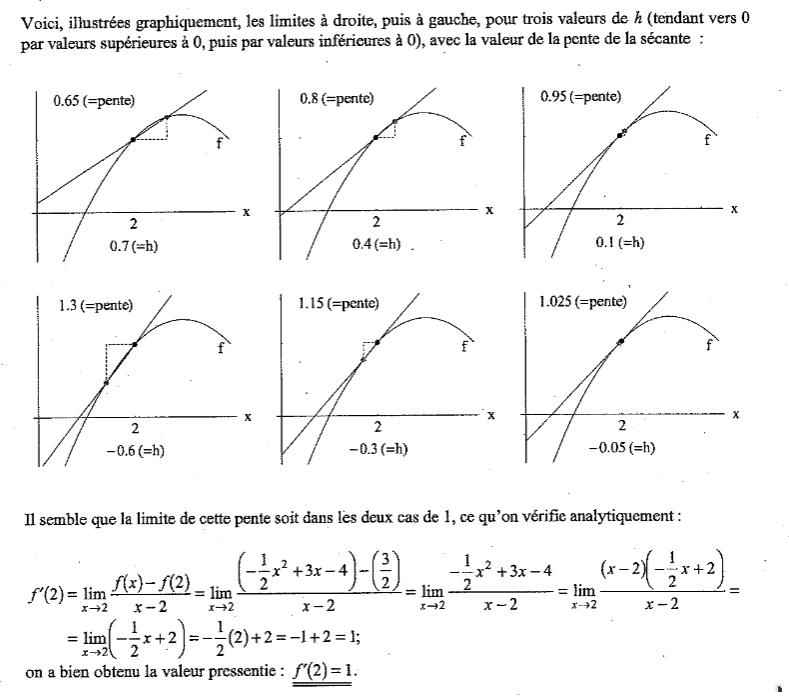
\includegraphics{../medias/3M/derivation/tangente}

\begin{remarque}
Interprétation géométrique
\tcblower
La dérivée d'une fonction $f$ en $a$ est égale, si elle existe, à la \textbf{pente de la tangente à la courbe représentative de} $f$ \textbf{au point} $(a;f(a))$.
\end{remarque}
\begin{exemple}
	calcul d'un nombre dérivé
	\tcblower
On considère la fonction $f$ définie par $f(x) = 3x^2$. À partir de la définition du nombre dérivé de $f$ en $-1$, calculer $f'(-1)$ et interpréter graphiquement.

$
\begin{aligned}
f'(-1) &= \displaystyle\lim_{h \to 0} \dfrac{f(-1 + h) - f(-1)}{h}\\
&= \displaystyle\lim_{h \to 0} \dfrac{3(-1 + h)^2 - 3(-1)^2}{h}\\
&= \displaystyle\lim_{h \to 0} \dfrac{3(h^2 - 2h + 1) - 3 \cdot 1}{h}\\
&= \displaystyle\lim_{h \to 0} \dfrac{3h^2 - 6h + 3 - 3}{h}\\
&= \displaystyle\lim_{h \to 0} \dfrac{3h^2 - 6h}{h}\\
&= \displaystyle\lim_{h \to 0} \dfrac{3h(h - 2)}{h}\\
&\stackrel{car h \neq 0}{=} \displaystyle\lim_{h \to 0} 3(h - 2)\\
&\stackrel{PrL 7}{=} 3(-2) = -6
\end{aligned}
$
\end{exemple}
\begin{thm}
	continuité et dérivabilité
	\tcblower
	Soit $f$ une fonction dérivable en $x$, alors $f$ est continue en $x$.
\end{thm}
\begin{remarque}
	\tcblower
	Attention, la réciproque n'est pas valable comme nous le verrons avec un contre-exemple dans la section suivante. 
\end{remarque}
\section{Non dérivabilité}
\begin{autre}
	\tcblower
Certaines fonction peuvent ne pas être dérivables en certains points (certaines ne sont même pas dérivables en tous points!).
\end{autre}
\begin{exemple}
	$f(x)=|x|$
	\tcblower
On considère la fonction $f$ définie par $f(x)=|x|$.
La fonction $|x|$ s'appelle la valeur absolue de $x$; elle est définie par : 

\[|x|=\begin{cases} x, \text{ si } x \geq 0 \\ -x, \text{ si } x<0 \end{cases}\]
On souhaite déterminer le nombre dérivé de $f$ en $0$. 

\[f'(0)=\displaystyle\lim_{h \to 0} \dfrac{f(0+h)-f(0)}{h}=\displaystyle\lim_{h \to 0} \dfrac{|h|-0}{h}\]

Problème : la valeur absolue de $h$ est différente selon que $h$ soit positif ou négatif ; il faut considérer les limites à gauche et à droite. Calculons

$\displaystyle\lim_{h \to 0^+} \dfrac{|h|-0}{h}=\displaystyle\lim_{h \to 0^+} \dfrac{h-0}{h}=\displaystyle\lim_{h \to 0^+} \dfrac{h}{h}=\displaystyle\lim_{h \to 0^+} 1=1$ et

$\displaystyle\lim_{h \to 0^-} \dfrac{|h|-0}{h}=\displaystyle\lim_{h \to 0^-} \dfrac{-h-0}{h}=\displaystyle\lim_{h \to 0^-} \dfrac{-h}{h}=\displaystyle\lim_{h \to 0^-} -1=-1$.

\end{exemple}
\begin{exemplesuite}
	\tcblower
On en conclut que $\displaystyle\lim_{h \to 0} \dfrac{|h|-0}{h}$ n'existe pas, et donc que $f$ n'est pas dérivable en 0.

{\bfseries Interprétation graphique :} Cela correspond à un « pic » de la courbe représentative de $f$.

En tendant vers 0 par la droite, la pente de la tangente (à $f$ en (0;0)) vaut toujours 1 alors que par la gauche, elle vaut toujours -1 !

Remarquons également que la tangente et la courbe de la représentative de la fonction sont confondues quand $x$ tend vers 1 par la gauche puis par la droite.
\end{exemplesuite}
\begin{remarque}
\tcblower	
Plus généralement, tout point anguleux dans la courbe représentative d'une fonction indique un point de non dérivabilité.
\end{remarque}
\begin{exemple}
	$f(x)=\begin{cases} 2&  x \leq 1 \\ -x+1 & x>1 \end{cases}$
	\tcblower
	Justifier graphiquement pourquoi la fonction $f$ définie par \[f(x)=\begin{cases} 2 & x \leq 1 \\ -x+1 & x>1 \end{cases}\] n'est pas dérivable en 1.

On remarque qu'en tendant vers $1$ par la droite, la pente de la tangente (à $f$ en $(1;f(1))$) est égale à $0$ ; par contre, en tendant vers $1$ par la gauche, elle vaut $-1$ !

La dérivée n'existe donc pas en 1.
\end{exemple}

\section{Fonction dérivée}

\begin{definition}
	fonction dérivée
	\tcblower
Soit une fonction $f : I \to \mathbb{R}$ dérivable en tout $a \in I$.
On appelle {\bfseries fonction dérivée} de la fonction $f$, ou plus simplement {\bfseries dérivée de $f$}, la fonction $f'$ qui à chaque $x \in I$ fait correspondre la dérivée de $f$ en $x$, soit
$f' : \begin{array}{ccc} I & \to & \mathbb{R} \\ x & \mapsto & f'(x) \end{array}$

Plus précisément, $f'$ est définie ainsi:

$f'$ est la fonction $f' : I \to \mathbb{R}$ telle que $f'(x)=\displaystyle\lim_{h \to 0} \dfrac{f(x+h)-f(x)}{h}$
\end{definition}

\begin{exemple}
	dérivée de $f(x)=3x^2$
	\tcblower
On considère la fonction $f$ définie par $f(x)=3x^2$. Déterminer $f'(x)$ à partir de la définition de la (fonction)

$\begin{aligned}
	f'(x)&=\displaystyle\lim_{h \to 0} \dfrac{f(x+h)-f(x)}{h} = \displaystyle\lim_{h \to 0} \dfrac{3(x+h)^2-3x^2}{h} \\
	     &=\displaystyle\lim_{h \to 0} \dfrac{3(x^2+2xh+h^2)-3x^2}{h}
= \displaystyle\lim_{h \to 0} \dfrac{3x^2+6xh+3h^2-3x^2}{h}\\
	     &= \displaystyle\lim_{h \to 0} \dfrac{6xh+3h^2}{h} = \displaystyle\lim_{h \to 0} \dfrac{3h(2x+h)}{h}
\stackrel{h \neq 0}{=} \displaystyle\lim_{h \to 0} 3(2x+h)\\
	     &= 3(2x+0)=6x
\end{aligned}$
\end{exemple}
\section{Représentation graphique de la dérivée}
\begin{methode}
	Représentation graphique de la dérivée
	\tcblower
Soit une fonction $f : I \to \mathbb{R}$ dont on donne une représentation graphique. On demande de représenter graphiquement dans le même repère sa dérivée~:
\begin{tasks}
\task On identifie les points de tangente horizontale ; ils correspondent à des dérivées nulles ;
\task on identifie d'éventuels intervalles où la pente de la tangente est facilement calculable (f constante ou affine) ; cela correspond à des valeurs constantes de la dérivée ;
\task on identifie les intervalles où la pente de la tangente est positive (ou négative) ; la dérivée sera positive (ou négative) ;
\task on estime quelques pentes de tangentes intéressantes qu'on reporte comme valeurs de la dérivée.
\end{tasks}
\end{methode}
\section{Équation de la tangente}

\begin{thm}
	Equation de la tangente
	\tcblower
Soit une fonction $f : I \to \mathbb{R}$ dérivable en tout $a \in I$.
L'équation de la tangente à $f$ au point $(a;f(a))$ est donnée par :
\[
y=f'(a)(x-a)+f(a)
\]
\end{thm}

\begin{exemple}
	équation de la tangente \\
	$f(x)=3x^2$
	\tcblower
On considère la fonction $f$ définie par $f(x)=3x^2$. Déterminer l'équation de la tangente en $(-1;f(-1))$.

Nous avons déjà calculé plus haut que $f'(-1)=-6$, et on a $f(-1)=3$.

On a donc : $y=-6(x-(-1))+3=-6x-3$.

Remarquons que sans connaître la formule générale, on aurait aussi pu procéder ainsi : comme $f'(-1)=-6$, on sait que $y=6x+q$. On a aussi : $f(-1)=3$, ce qui signifie que $3=-6(-1)+q \Rightarrow 3=6+q$ et donc $y=-6x-3$
\end{exemple}

\section{Bilan intermédiaire}

\begin{autre}
	\tcblower
Nous avons pu dans les exercices, à l'aide de la définition de la dérivée, déterminer la dérivée $f'$ d'un certain nombre de fonctions $f$ données.
\end{autre}

\begin{notation}
dérivée
\tcblower
Si on doit déterminer la (fonction) dérivée de la fonction $f$, par exemple définie par $f(x)=x^3+3x$, on écrira plus simplement $(x^3+3x)'=\ldots$
\end{notation}


\begin{formule}
Dérivées de fonctions élémentaires
	\tcblower
	On a les formules de dérivation suivantes des fonctions élémentaires
	\begin{multicols}{2}
	\begin{description}
  \item[D1] $(\text{cte})'=0$
  \item[D2] $(x)'=1$
  \item[D3] $(ax+b)'=a$
  \item[D4] $(x^2)'=2x$
  \item[D5] $(ax^2+bx+c)'=2ax+b$
  \item[D6] $(x^3)'=3x^2$
  \item[D7] $\bigl(\sqrt{x}\bigr)'=\dfrac{1}{2\sqrt{x}}$
  \item[D8] $\left(\dfrac{1}{x}\right)'=-\dfrac{1}{x^2}$
\end{description}
\end{multicols}
\end{formule}
\begin{exemple}
	Quelques calculs de dérivées
	\tcblower
	\begin{tasks}(2)
		\task $(x^3)'=x^{3-1}=x^2$ 
		\task $(x^{23})'=23x^{23-1}=x^{22}$
		\task $(x^{-2})'=x^{-2-1}$
		\task $(x^{-5})'=-5x^{-5-1}=-5x^{-6}$
	\end{tasks}

\end{exemple}

\section{Formules de dérivation}

\begin{formule}
Formules de dérivation
\tcblower
On a la formules suivantes~:
\begin{description}
\item [PrD1] $[cte]' = cte \cdot f'$
\item [PrD2] $[f + g]' = f' + g'$  
\item [PrD3] $[f - g]' = f' - g'$
\item [PrD4] $[f \cdot g]' = f' \cdot g + f \cdot g'$
\item [PrD5] $\left[\dfrac{1}{f}\right]' = -\dfrac{f'}{f^2}$
\item [PrD6] $\left[\dfrac{f}{g}\right]' = \dfrac{f' \cdot g - f \cdot g'}{g^2}$
\item [PrD7] $\left[\dfrac{cte}{f}\right]' = -\dfrac{cte \cdot f'}{f^2}$
\item [PrD8] $[f(x)]^n = n[f(x)^{n-1}] \cdot f'(x), \forall n \in \mathbb{R}$
\item [PrD9] $[g(f(x))]' = g'(f(x)) \cdot f'(x)$
\end{description}
\end{formule}

\begin{remarque}
	\tcblower
Nous acceptons pour le moment ces formules sans les démontrer. Nous y reviendrons plus loin et il faudra alors être capable de les énoncer puis de les démontrer sous forme de théorèmes !
\end{remarque}

\begin{formule}
dérivées de fonctions élémentaires - suite
\tcblower
Avec les formules précédentes, on peut montrer :
\begin{description}
\item[D9] $[x^n]' = nx^{n-1}, \forall n \in \mathbb{R}$
\end{description}
\end{formule}

\begin{exemple}
	dérivée de $f(x)=3x$
	\tcblower
$(3x)' \stackrel{\text{PrD1}}{=} 3(x)' \stackrel{\text{D1}}{=} 3 \cdot 1 = 3$
\end{exemple}

\begin{exemple}
	dérivée de $g(x)=ax^2+bx+c$
	\tcblower
$\begin{aligned}
	(ax^2 + bx + c)' &\stackrel{\text{PrD2}}{=} (ax^2)' + (bx)' + (c)'\\ &\stackrel{\text{D1 et PrD1}}{=} a(x^2)' + b(x)' + 0\\
			 &\stackrel{\text{D4 et D1}}{=} a(2x) + b \cdot 1\\
			 &= 2ax + b
\end{aligned}$
\end{exemple}

\section{Extrema de $f$ et points critiques}

\begin{definition}
	maximum et minimum
\tcblower
Soit $f$ définie sur un intervalle $I$ et $x \in I$

$f$ admet un \textbf{minimum (local)} en $a \Leftrightarrow \exists$ un voisinage $V$ de $a$ tel que 

$f(a) \leq f(x), \forall x \in V$

$f$ admet un \textbf{maximum (local)} en $a \Leftrightarrow \exists$ un voisinage $V$ de $a$ tel que 

$f(a) \geq f(x), \forall x \in V$

$f$ admet un \textbf{minimum global} en $a \Leftrightarrow f(a) \leq f(x), \forall x \in D_f$

$f$ admet un \textbf{maximum global} en $a \Leftrightarrow f(a) \geq f(x), \forall x \in D_f$

\end{definition}
\begin{remarque}
	\tcblower
Désormais, lorsqu'on parlera de minimum ou de maximum, sans plus de précision, on pensera toujours minimum ou maximum local.
\end{remarque}
\begin{definition}
	point critique
	\tcblower
	Soit une fonction $f$ définie sur un ensemble $I$. On appelle $a\in I$ un {\bfseries point critique} si $f$ est dérivable en $a$ et $f'(a)=0$.
\end{definition}

\begin{remarque}
	conjecture fausse
	\tcblower
	Soit $f:\mathbb{R}\rightarrow \mathbb{R}$ et $a\in \mathbb{R}$ tel que $f$ admet un extremum local en $a$, alors $f'(a)=0$.

	{\bfseries Contre-exemple~:} $f(x)=|x|$ et $a=0$. 
\end{remarque}


\begin{remarque}
	conjecture fausse
	\tcblower
	Soit $f:\mathbb{R}\rightarrow \mathbb{R}$ et $a\in \mathbb{R}$ tel que $f'(a)=0$, alors f admet un extremum local en $a$.

	{\bfseries Contre-exemple~:} $f(x)=x^3$ et $a=0$. 
\end{remarque}

\begin{thm}
	extremum local
	\tcblower
	Si $f:\mathbb{R}\rightarrow \mathbb{R}$ et $a\in \mathbb{R}$ tel que $f$ est dérivable en $a$ et $f$ admet un extremum local en $a$, alors $f'(a)=0$.
\end{thm}
\begin{remarque}
zéros de la dérivée
\tcblower
Il existe des fonctions $f$ pour lesquelles $f'(a) = 0$ et $f$ n'admet pas d'extremum en $a$, ou $f'(a) = 0$ et $f$ admet un extremum en $a$. La « simple » connaissance des zéros de la dérivée $f'$ ne suffit donc pas à pouvoir affirmer avec certitude que ceux-ci sont des extrema locaux de $f$ ! Pour une fonction dérivable, l'ensemble des points critiques de $f$ contient mais n'est pas forcément égal à celui des zéros de $f'$.

Lorsque la fonction est dérivable, il faut toujours faire le tableau de signes complet de la dérivée pour pouvoir bien comprendre la situation. Autrement, la section suivante nous permet de tirer des conclusion si la fonction est {\bfseries continue}.
\end{remarque}
\section{Théorème de Rolle et des accroissements finis}
\begin{thm}
Thm de Rolle
\tcblower
Si $f : I \to \mathbb{R}$ est telle que :
\begin{itemize}
\item $f$ est continue sur $[a,b]$
\item $f$ est dérivable sur $]a,b[$
\item $f(a) = f(b)$
\end{itemize}
alors il existe au moins un nombre $c \in ]a,b[$ tel que $f'(c) = 0$.
\end{thm}
\begin{thm}
Thm des accroissement finis
\tcblower
Si $f : I \to \mathbb{R}$ est telle que :
\begin{itemize}
\item $f$ est continue sur $[a,b]$
\item $f$ est dérivable sur $]a,b[$
\end{itemize}
alors il existe au moins un nombre $c \in ]a,b[$ tel que $f'(c) = \dfrac{f(b) - f(a)}{b - a}$
\end{thm}

\section{Signe de $f'$ et monotonie de $f$}
\begin{autre}
	\tcblower
	Dans cette section, nous déduisons des corrollaires au théorème des accroissements finis.
\end{autre}
\begin{definition}
	croissance\\
	décroissance
	\tcblower
Soit $f$ définie sur un intervalle $I$.

On dit que $f$ est \textbf{croissante} sur $I$ si 

$\forall x,y\in I$ tels que $x>y$, on a $f(x) \geq f(y)$.

On dit que $f$ est \textbf{strictement croissante} sur $I$ si

$\forall x,y\in I$ tels que $x>y$, on a $f(x) > f(y)$.

On dit que $f$ est \textbf{décroissante} sur $I$ si

$\forall x,y\in I$ tels que $x>y$, on a $f(x) \leq f(y)$.

On dit que $f$ est \textbf{strictement décroissante} sur $I$ si

$\forall x,y\in I$ tels que $x>y$, on a $f(x) < f(y)$.
\end{definition}
\begin{thm}
	monotonie et dérivée\\
	corollaire des accroissements finis
	\tcblower
Soit $f$ dérivable sur un intervalle $I$. Alors on a :
\begin{itemize}
	\item si $f'(x) > 0, \forall x \in I$, alors $f$ est croissante sur $I$
\item si $f'(x) < 0, \forall x \in I$, alors $f$ est décroissante sur $I$
\item si $f'(x) = 0, \forall x \in I$, alors $f$ est constante sur $I$
\end{itemize}
\end{thm}
\begin{remarque}
	\tcblower
	Ce théorème nous permet de résoudre des problèmes d'optimisation et d'étudier complètement des fonctions. Nous en ferons bon usage dans les parties \ref{sec:opti} et \ref{sec:etude}.
\end{remarque}
\begin{thm}
réciproque du corollaire des accroissement finis
\tcblower
Soit $f$ définie sur un intervalle $I$.
Alors on a :
\begin{itemize}
\item si $f$ est strictement croissante sur $I$, alors $f'(x) > 0, \forall x \in I$
\item si $f$ est strictement décroissante sur $I$, alors $f'(x) < 0, \forall x \in I$
\item si $f$ est constante sur $I$, alors $f'(x) = 0, \forall x \in I$
\end{itemize}
\end{thm}
\begin{exemple}
	monotonie de $f(x)=x^3-6x^2+9x-4$
	\tcblower
Étudier la monotonie de la fonction $f$ définie par $f(x) = x^3 - 6x^2 + 9x - 4$ puis la représenter graphiquement.

on calcule la dérivée : $(x^3 - 6x^2 + 9x - 4)' = 3x^2 - 12x + 9$

on la factorise : $f'(x) = 3(x^2 - 4x + 3) = 3(x - 1)(x - 3)$

on construit le tableau de signes de $f'(x)$ :
\begin{center}
\begin{tabular}{|c|c|c|c|c|c|}
\hline
$x$ & & 1 & & 3 & \\
\hline
3 & + & + & + & + & + \\
\hline
$(x-1)$ & - & 0 & + & + & + \\
\hline
$(x-3)$ & - & - & - & 0 & + \\
\hline
$f'(x)$ & + & 0 & - & 0 & + \\
\hline
$f(x)$ & $\nearrow$ & max & $\searrow$ & min & $\nearrow$ \\
\hline
\end{tabular}
\end{center}

La dernière ligne du tableau donne la monotonie de $f$.

On calcule les points critiques, ici ses extrema : $f(1) = -0$ et $f(3) = -4$.

On détermine encore, pour produire une représentation graphique de $f$ :
\begin{itemize}
	\item l'ordonnée à l'origine : $f(0) = -4$
	\item les zéros : on cherche parmi les diviseurs de 4 et on trouve $f(1) = f(4) = 0$ ; on utilise la division polynomiale par $(x - 1)(x - 4) = x^2 - 5x + 4$ et on trouve $f(x) = (x - 1)^2(x - 4)$, d'où $Z_f = \{1; 4\}$
\end{itemize}
\end{exemple}

\begin{exemple}[label=ex:premder]
	monotonie de\medskip

	$f(x)=\dfrac{1}{4}x^4-\dfrac{4}{3}x^3+2x^2$
	\tcblower
	Étudier la monotonie de la fonction $f$ définie par $f(x) = \dfrac{1}{4}x^4 - \dfrac{4}{3}x^3 + 2x^2$ puis la représenter graphiquement.

On calcule la dérivée : $\left(\dfrac{1}{4}x^4 - \dfrac{4}{3}x^3 + 2x^2\right)' = x^3 - 4x^2 + 4x$

On cherche les zéros de la dérivée : $x^3 - 4x^2 + 4x = 0 \Leftrightarrow x(x^2 - 4x + 4) = 0 \Leftrightarrow x(x - 2)^2 = 0$

On construit le tableau de signes de $f'(x)$ :
\begin{center}
\begin{tabular}{|c|c|c|c|c|c|}
\hline
$x$ & & 0 & & 2 & \\
\hline
$x$ & - & 0 & + & + & + \\
\hline
$(x-2)^2$ & + & + & + & 0 & + \\
\hline
$f'(x)$ & - & 0 & + & 0 & + \\
\hline
$f(x)$ & $\searrow$ & min & $\nearrow$ & & $\nearrow$ \\
\hline
\end{tabular}
\end{center}
On a 

$f(x) = \dfrac{1}{4}x^4 - \dfrac{4}{3}x^3 + 2x^2 = x^2\left(\dfrac{1}{4}x^2 - \dfrac{4}{3}x + 2\right) = \dfrac{1}{12}x^2(3x^2 - 16x + 24)$

$3x^2 - 16x + 24$ n'est pas factorisable, car $\Delta = -32$, donc $Z_f = \{0\}$


\end{exemple}


\section{Deuxième dérivée}
\begin{definition}
	convexité et concavité\\
	intuitivement et formellement
	\tcblower
	{\bfseries Définition intuitive}

Soit $f$ définie sur un intervalle $I$.

On dit que $f$ est \textbf{convexe} sur $I$ si le segment le segment joignant $(a ;f(a))$ à $(b ;f(b))$ «passe au-dessus du graphe de $f$», $\forall a, b \in I$

On dit que $f$ est \textbf{concave} sur $I$ si le segment le segment joignant $(a ;f(a))$ à $(b ;f(b))$ «passe au-dessous du graphe de $f$», $\forall a, b \in I$

\textbf{Définition formelle}

Considérons la situation de convexité précédente : on note $A(a ;f(a))$, $B(b ;f(b))$ et $C(x ;f(x))$.

La pente du segment $s_1=[AB]$ est égale à $\dfrac{f(b) - f(a)}{b - a}$ et celle de $s_2=[AC]$ vaut $\dfrac{f(x) - f(a)}{x - a}$.

$f$ est (strictement) \textbf{convexe} sur $I$ si et seulement si on a :
$\dfrac{f(x) - f(a)}{x - a} < \dfrac{f(b) - f(a)}{b - a}$ $\forall a, x, b \in I$ avec $a < x < b$

$f$ est (strictement) \textbf{concave} sur $I$ si et seulement si on a :
$\dfrac{f(x) - f(a)}{x - a} > \dfrac{f(b) - f(a)}{b - a}$ $\forall a, x, b \in I$ avec $a < x < b$

\end{definition}

\begin{remarque}
	strictement!
	\tcblower
Contrairement aux notions de minimum/maximum/(dé)croissance où on travaille avec des «plus petit/grand ou égal» dans les définitions, on exclut ici la situation limite d'une droite qui n'est alors ni convexe, ni concave.
\end{remarque}

\begin{definition}
	deuxième dérivée
	\tcblower
Soit $f$ définie sur un intervalle $I$.

La \textbf{deuxième dérivée} $f''$ de $f$ (ou \textbf{dérivée seconde}) est la dérivée de $f'$
\end{definition}

\begin{definition}
	domaine de concavité
	\tcblower
	Soit $f$ une fonction définie sur un ouvert $I$. On dit que $J\subset I$ est un {\bfseries domaine de concavité} si $f$ est concave sur $J$. 
\end{definition}

\begin{definition}
	domaine de convexité
	\tcblower
	Soit $f$ une fonction définie sur un ouvert $I$. On dit que $J\subset I$ est un {\bfseries domaine de convexité} si $f$ est convexe sur $J$. 
\end{definition}

\begin{definition}
	point d'inflexion
	\tcblower
Un \textbf{point d'inflexion} de $f$ sépare un domaine de concavité d'un domaine de convexité.
\end{definition}
\begin{thm}
point d'inflexion
\tcblower
Soit $f$ deux fois dérivable sur un intervalle $I$. Alors on a :
\begin{itemize}
	\item si $f''(x) > 0, \forall x \in I$, alors $f$ est convexe sur $I$
	\item si $f''(x) < 0, \forall x \in I$, alors $f$ est concave sur $I$
\end{itemize}
\end{thm}
\begin{remarque}
	zéros de la deuxième dérivée
	\tcblower
Il existe des fonctions $f$ pour lesquelles $f''(a) = 0$ et $f$ n'admet pas de point d'inflexion en $a$, ou $f''(a) = 0$ et $f$ admet un point d'inflexion en $a$. La « simple » connaissance des zéros de la deuxième dérivée $f''$ ne suffit donc pas à pouvoir affirmer avec certitude que ceux-ci sont des points d'inflexion de $f$ ! Lorsque la fonction est deux fois dérivable, il faut toujours faire le tableau de signes complet de la deuxième dérivée pour pouvoir bien comprendre la situation.
\end{remarque}
\begin{exemple}
	Esquisser $f(x)=\dfrac{1}{4}x^4-\dfrac{4}{3}x^3+2x^2$  
	\tcblower
On considère à nouveau la fonction de l'exemple \ref{ex:premder} 
\[f(x)=\dfrac{1}{4}x^4-\dfrac{4}{3}x^3+2x^2\] 
On calcule sa deuxième dérivée 
TODO
\end{exemple}
\section{Optimisation}
\label{sec:opti}
Dans notre contexte, \textbf{optimiser} signifie déterminer les extrema d'une situation donnée.

\begin{methode}
optimisation
\tcblower
Pour résoudre un problème d'optimisation on suit les étapes suivantes~:
\begin{tasks}(1)
\task Identifier et nommer la(les) inconnue(s).
\task Identifier ce qui doit être optimisé et l'exprimer algébriquement à l'aide des inconnues.
\task Réduire l'expression à une unique inconnue en utilisant une ou plusieurs relation existant entre les différentes inconnues.
\task On a maintenant une fonction d'une seule variable qui mesure la quantité à optimiser
\task On dérive $f$.
\task On factorise $f'$.
\task On cherche le(s) zéro(s) de $f'$.
\task On fait le tableau de signes de $f'$.
\task On identifie la solution (pour toutes les inconnues).
\task On répond à la question, en tenant compte des unités.
\end{tasks}
\end{methode}

\begin{exemple}
	optimiser une somme
	\tcblower
Déterminer deux nombres positifs dont la somme vaut $8$ et dont la somme des carrés soit minimale.
\begin{tasks}
\task Soit $x$ et $y$ les deux nombres.
\task La somme des cubes à optimiser : $x^2 + y^2$.
\task $x + y = 8$, donc $y = 8 - x$
\task d'où la somme des cubes en fonction de $x$ seul : $f(x) = x^2 + (8 - x)^2$ 
\task  Dérivée : $f'(x) = (x^2 + (8 - x)^2)' = 2x + 2(8 - x)(-1) = 2x - 2(8 - x) = 4x - 16$
\task Factorisation : $f'(x) = 4(x - 4)$
\task Zéros de la dérivée : $Z_{f'} = \{4\}$
\task Tableau de signes de la dérivée :
\begin{center}
\begin{tabular}{|c|c|c|c|}
\hline
$x$ & & 4 & \\
\hline
$f'(x)$ & - & 0 & + \\
\hline
$f(x)$ & $\searrow$ & min & $\nearrow$ \\
\hline
\end{tabular}
\end{center}
\task  $x = 4$, d'où $y = 8 - 4 = 4$
\task Les deux nombres sont 4 et 4.
\end{tasks}
\end{exemple}

\section{Étude de fonction}

\label{sec:etude}
\begin{methode}
	étude de fonction
	\tcblower
\textbf{Étudier une fonction}, c'est :
\begin{tasks}(1)
\task Déterminer $D_f$.
\task Déterminer les intersections avec les axes, soit $f(0)$ et $Z_f$ (facultativement son tableau de signes).
\task Déterminer toutes les asymptotes.
\task Calculer la dérivée.
\task La factoriser.
\task Déterminer les zéros de $f'$.
\task Établir le tableau de signes de $f'$ et le tableau de variations de $f$.
\task En déduire les points critiques de $f'(x)$ (deux coordonnées).
\task * Selon les indications de l'énoncé calculer ou non la deuxième dérivée, la factoriser, déterminer ses zéros et son tableau de signes ; en déduire la concavité/convexité de $f$ et les points d'inflexion.
\task Représenter graphiquement $f$ en utilisant toutes les informations récoltées jusque-là (si nécessaire en calculant encore quelques images pour augmenter la précision du tracé).
\end{tasks}
\end{methode}

\begin{exemple}
Étude de la fonction\\
\medskip
$f(x) = \dfrac{x^2-1}{x^2-3x-4}$
\tcblower	
Étudier la fonction $f$ définie par $f(x) = \dfrac{x^2-1}{x^2-3x-4}$.

On a : 
\begin{equation}
	f(x) = \dfrac{x^2-1}{x^2-3x-4} = \dfrac{(x-1)(x+1)}{(x-4)(x+1)} \stackrel{x\neq -1}{=} \dfrac{x-1}{x-4} \label{eq:simpl}\tag{$\star$}
\end{equation}
cette dernière simplification est très utile; partout où l'on est certain que $x$ est différent de $1$, on peut travailler avec l'expression $\dfrac{x-1}{x-4}$ qui est bien plus simple à manipuler !

On suit chaque étape selon la méthode ci-dessus.
\begin{tasks}
	\task On exclut les valeurs qui annulent $(x-4)(x+1)$, c'est-à-dire si $x = -1$ ou $x = 4$, donc $D_f = \mathbb{R} \setminus \{-1;4\}$
	\task $f(0) = \dfrac{1}{4}$ et $f(x) = 0 \Leftrightarrow 1-x^2 = 0$ (et $x \in D_f$) $\Leftrightarrow (x-1)(1+x) = 0$ (et $x \in D_f$), donc $Z_f = \{1\}$
	\task En considérant l'équation (\ref{eq:simpl}), on voit immédiatement que $f$ admet une asymptote verticale en $x = 4$ (limite du type $\dfrac{1}{0}$), un « trou » en $x = -1$ (limite du type $\dfrac{0}{0} \rightarrow$ simplifier $\rightarrow$ calculer) et une asymptote horizontale $y = 1$ à $\pm\infty$ (même degré au numérateur et au dénominateur)

Dans tous les cas, on calcule la limite de type $\dfrac{0}{0}$~:
\[\displaystyle\lim_{x \to -1} f(x) = \displaystyle\lim_{x \to -1} \dfrac{x-1}{x-4} = \dfrac{-1-1}{-1-4} = \dfrac{2}{5}.\]

On calcule également les limites à gauche et à droite pour $x\to 4$. On obtient par (\ref{eq:simpl}), $\displaystyle\lim_{x\to 4^-}f(x)=-\infty$ et $\displaystyle\lim_{x\to 4^+}f(x)=+\infty$ 

On connaît également le comportement à $\pm\infty$, car la fonction admet une asymptote horizontale déterminée précédemment.

\task 
On calcule la dérivée 

$\begin{aligned}
	f'(x) &= \dfrac{x^2-1}{(x^2-3x-4)'}\\
	      &\stackrel{x\neq 1}{=} \left(\dfrac{x-1}{x-4}\right)\\
	      &= \dfrac{1 \cdot (x-4)-(x-1) \cdot 1}{(x-4)^2}\\
	      &= \dfrac{x-4-x+1}{(x-4)^2}\\
	      &= \dfrac{-3}{(x-4)^2}
\end{aligned}
$
\task  $f'$ est déjà factorisée

\task  Zéros de $f'$: $Z_{f'} = \emptyset$

\task Tableau de signes de la dérivée (attention de ne pas oublier $x = -1$ dans le tableau!) :
\begin{center}
$
\begin{array}{c|c|c|c|c|c}
x & & -1 & & 4 & \\
\hline
-3 & - & & - & & - \\
\hline
(x-4)^2 & + & & + & 0 & + \\
\hline
f'(x) & - & /// & - & /// & - \\
\hline
f(x) & \searrow & /// & \searrow & /// & \searrow
\end{array}
$
\end{center}
\task pas de points critiques

\task $f''(x) = \dfrac{d}{dx}\left[\dfrac{-3}{(x-4)^2}\right] = -3 \cdot \dfrac{1}{(x-4)^2} = -3 \cdot \dfrac{-(x-4)^2)'}{(x-4)^4} = -3 \cdot \dfrac{-2(x-4)}{(x-4)^4}$

$= \dfrac{6(x-4)}{(x-4)^4} = \dfrac{6}{(x-4)^3}$

Zéros de $f''$: $Z_{f''} = \emptyset$
\begin{center}
$
\begin{array}{c|c|c|c|c|c}
x & & -1 & & 4 & \\
\hline
6 & + & & + & + & + \\
\hline
(x-4)^3 & - & & - & 0 & + \\
\hline
f''(x) & + & /// & + & /// & - \\
\hline
f(x) & \text{concave} & /// & \text{concave} & /// & \text{convexe}
\end{array}
$
\end{center}
\end{tasks}
\end{exemple}

\section{Exercices}


\insertexo{1M-y1c7r}{true}{exo}{true}
\insertexo{1M-c6eaz}{true}{exo}{true}

\insertexo{1M-1h2rj}{true}{exo}{true}
\insertexo{1M-bv651}{true}{exo}{true}
\insertexo{1M-1h1tt}{true}{exo}{true}
\insertexo{1M-t3pgp}{true}{exo}{true}
\insertexo{1M-r98sf}{true}{exo}{true}
\insertexo{1M-51tvf}{true}{exo}{true}
\insertexo{1M-ju5sg}{true}{exo}{true}
\insertexo{1M-ttwes}{true}{exo}{true}
\insertexo{1M-yazhe}{true}{exo}{true}
\insertexo{1M-rv1yv}{true}{exo}{true}
\insertexo{1M-vnbfx}{true}{exo}{true}
\insertexo{1M-ryapx}{true}{exo}{true}
\insertexo{1M-zeeed}{true}{exo}{true}
\insertexo{1M-gv9rr}{true}{exo}{true}
\insertexo{1M-fcxr6}{true}{exo}{true}
\insertexo{1M-8wcq9}{true}{exo}{true}
\insertexo{1M-vrkth}{true}{exo}{true}
\insertexo{1M-y4385}{true}{exo}{true}
\insertexo{1M-2at6d}{true}{exo}{true}
\insertexo{1M-mj5qq}{true}{exo}{true}
\insertexo{1M-hgcu8}{true}{exo}{true}
\insertexo{1M-y4dv7}{true}{exo}{true}
\insertexo{1M-ek51g}{true}{exo}{true}
\insertexo{1M-5en1r}{true}{exo}{true}
\insertexo{1M-1gayt}{true}{exo}{true}
\insertexo{1M-955md}{true}{exo}{true}
\insertexo{1M-g4sjk}{true}{exo}{true}
\insertexo{1M-b3p6g}{true}{exo}{true}
\insertexo{1M-hzaw5}{true}{exo}{true}
\insertexo{1M-uyvgj}{true}{exo}{true}
\insertexo{1M-qsgvn}{true}{exo}{true}
\insertexo{1M-kksbd}{true}{exo}{true}
\insertexo{1M-c3ghj}{true}{exo}{true}
\insertexo{1M-meks3}{true}{exo}{true}

\subsection{Limites trigonométriques}
\insertexo{1M-u68mh}{true}{exo}{true}
\insertexo{1M-areny}{true}{exo}{true}
\insertexo{1M-hhksj}{true}{exo}{true}
\subsection{thm formules}
\subsection{thm importants}

\end{document}
